\section{Anticipatory defense on the choice of test environments and metrics}
\label{app_sec:ant_defense_test_env}

% 主动承认并界定研究范围：明确指出，本工作的首要目标是机理研究，而非追求极致的现实仿真。Mini-BEHAVIOR在保留家庭任务的长视距、多对象、状态依赖等高层级决策复杂性的同时，主动剥离了低层级感知与控制的噪音。这使我们能够将模型失败更清晰地归因于语言grounding和规划问题，而非纹理识别或连续运动控制。

% 使用“先理解，再扩展”的研究范式论证：引用经典研究范式——先在受控的简化环境中理解核心机理，再将验证过的假设推广到更复杂的场景。可以说明，我们的形式化方法（规则宽度）是任务和平台无关的，未来可以在更复杂的仿真器中复用同一套指令生成与控制框架。

% 对比优势：简要对比指出，在iGibson等高级仿真器中，难以程序化地生成海量、精确对应不同规则宽度的指令-轨迹对，且渲染和物理计算成本过高，不利于进行需要大量实验迭代的消融研究。

In this work, we selected Mini-BEHAVIOR as our testbed. This choice is motivated by several key considerations aligned with our research objectives. Our research objective is not to solve the full stack of robotic embodiment (which includes perception, continuous control, and physics), but specifically to isolate and analyze the impact of instruction granularity on language grounding and long-horizon planning.

Therefore, high-fidelity simulators (e.g., iGibson \citep{li2022igibson}, BEHAVIOR-1K \citep{DBLP:conf/corl/0002ZWGSMWLLSAH22}) introduce significant noise through complex texture rendering and continuous motor control. While realistic, these factors act as confounders. When an agent fails in such environments, it is often difficult to attribute the failure to a lack of linguistic understanding (granularity issues) or a failure in low-level execution (e.g., grasping physics or occlusion). Mini-BEHAVIOR retains the high-level decision complexity of household tasks—long horizons, multi-object interactions, and state dependencies—while abstracting away low-level sensorimotor noise.

In the perspective of fast prototyping and iterative experimentation, we have to also consider the rendering and physics simulation costs. Mini-BEHAVIOR's grid-based discrete control and simplified visual representation allow for rapid data generation and model training. 

Another consideration is the diversity of the task structures so that we can systematically vary instruction granularity across a wide range of scenarios. As such, Crafter \citep{hafner2021crafter}, which focuses on survival in a single domain, lacks the diverse task structures needed to obtain robust insights about instruction granularity. 

Table \ref{tab:env_comparison} provides a detailed comparison of Mini-BEHAVIOR against other prominent benchmarks, highlighting why they were less suitable for this specific investigation.

\begin{table*}[t]
\small
\centering
\caption{Comparison of Embodied AI Environments regarding their suitability for studying Instruction Granularity.}
\label{tab:env_comparison}
\begin{tabular}{@{}l>{\raggedright\arraybackslash}p{1.4cm}c>{\raggedright\arraybackslash}p{1.5cm}>{\raggedright\arraybackslash}p{1.7cm}>{\raggedright\arraybackslash}p{4.9cm}@{}}
\toprule
\textbf{Environment} & \textbf{Control} & \textbf{Horizon} & \textbf{Visuals} & \textbf{Symbolic Abstraction} & \textbf{Limitation} \\
\midrule
\textbf{Mini-BEHAVIOR}(*) & Discrete & Long & Grid & \textbf{Support} & \textbf{Ideal balance:} Supports symbolic state abstraction; diverse task suite; removes control noise while retaining logic complexity. \\
\textbf{Crafter} & Discrete & Long & Cartoon & Partial & Single task suite (survival); partially observable (memory heavy); few object types. \\
\textbf{Meta-World} & Continuous & Short & 3D & No & Continuous control; no symbolic abstraction; focus on multi-task RL/manipulation, not long-horizon planning. \\
\textbf{LIBERO} & Continuous & Short & 3D & No & Robotic arm focus; continuous control; no symbolic abstraction; VLA success rate already saturated (tasks relatively easy). \\
\textbf{RoboTwin 2.0} & Continuous & Short & 3D & No & Continuous control; no symbolic abstraction; dual-arm manipulation focus; hard to segment expert trajectories and construct granular instructions. \\
\textbf{CALVIN} & Continuous & Medium & 3D & No & Hard to design instruction granularity due to continuous action space (though provides diverse language); confounds planning with control difficulties. \\
\textbf{ALFRED} & Discrete & Long & 3D Photo & Support & 3D partially observable; poor infrastructure support for VLA training; high rendering cost. \\
\textbf{iGibson / BEHAVIOR-1K} & Continuous & Long & 3D Photo & Partial & Good for long-horizon tasks, but 3D realistic vision context becomes a confounder. \\
\bottomrule
\end{tabular}%
\end{table*}

\section{Symbolic Representation of the Embodied Task}
\label{app_sec:classical_prob_def}


We formalize the Mini-BEHAVIOR environment as a deterministic grid-based symbolic world. This allows us to represent the challenge as a classical planning problem $\mathcal{P} = \langle \mathcal{F}, \mathcal{A}, s_0, G \rangle$, where:
\begin{itemize}[leftmargin=*]
    \item $\mathcal{F}$ is a finite set of propositional fluents representing the state variables of the environment (e.g., object locations, states like \textit{cooked} or \textit{open}).
    \item $\mathcal{A}$ is a finite set of actions available to the agent.
    \item $s_0 \subseteq \mathcal{F}$ is the initial state configuration.
    \item $G \subseteq \mathcal{F}$ is the goal condition that must be satisfied.
\end{itemize}
A state $s \in \mathcal{S}$ is defined as a truth valuation over $\mathcal{F}$, with the state space $\mathcal{S} \subseteq 2^\mathcal{F}$ encompassing all valid combinations of fluent truth values.

\section{Details of \textsc{Mini-BEHAVIOR} Environment}
\label{app_sec:minibehavior_details}

To operationalize our formalism, we developed a \textbf{Universal PDDL Domain Model} (available at \url{minibehavior_gran_domain_model.pddl} in the codebase) capable of supporting all 20 household tasks without modification. This unified model comprises over 1,000 lines of PDDL 2.1 definitions and is fully compatible with the LAMA planner. We highly recommend checking the codebase for the complete domain model.

\paragraph{Search Space Characteristics}
\begin{table}[H]
    \centering
    \small
    \caption{Planning complexity in typical tasks.}
    \label{tab:planning_complexity}
    \begin{tabular}{@{}lc@{}}
        \toprule
        \textbf{Metric} & \textbf{Typical Range} \\
        \midrule
        Objects & 15--40 \\
        Grid Locations & 20--60 \\
        Ground Actions & $10^3$--$10^5$ \\
        Plan Length & 50--200 primitive actions \\
        Planning Time (LAMA) & 0.5--300+ seconds \\
        \bottomrule
    \end{tabular}
\end{table}

\section{Details of \textsc{Mini-BEHAVIOR-Gran} Extension}
\label{app_sec:minibehavior_gran_details}

\textsc{Mini-BEHAVIOR} provides the foundational task skeletons, which we extend in \textsc{Mini-BEHAVIOR-Gran} to support multi-granularity instruction generation. A core component of this extension is the definition of a symbolic feature set used to generate rule-based policy sketches.


\subsection{Feature Categories}

The environment defines two primary categories of features: Boolean State Features and Quantitative Features.

\subsubsection{Boolean State Features}
These features evaluate whether a specific object instance satisfies a predicate. They require grounding (binding to specific object instances, e.g., \texttt{rag-01}).

\begin{table}[t]
\centering
\caption{Boolean State Features}
\label{tab:bool_features}
\resizebox{\columnwidth}{!}{%
\begin{tabular}{l|l|l}
\hline
\textbf{Feature} & \textbf{Applicable Objects} & \textbf{Semantics} \\ \hline
\texttt{Holding} & All Items & Is the agent holding the specified object? \\
\texttt{isOpened} & Cabinets, Drawers, Doors & Is the container/door open? \\
\texttt{isToggled} & Sinks, Stoves, Switches & Is the appliance turned on? \\
\texttt{isSoaked} & Rags, Sponges & Is the cleaning tool wet? \\
\texttt{isCleaned} & Shoes, Dishes, Floor & Is the object free of stains? \\
\texttt{isDustFree} & Furniture, Surfaces & Is the object free of dust? \\ \hline
\end{tabular}%
}
\end{table}

\subsubsection{Quantitative and Spatial Features}
These features capture distances, counts, and spatial relationships. Crucially, they support temporal comparison allowing conditions such as ``distance decreased'' or ``count dropped to zero.''

\begin{itemize}[leftmargin=*]
\item \textbf{\texttt{DistanceToNearest(type, condition)}}: Measures the Manhattan distance from the agent to the nearest object of a specific type.
\begin{itemize}[leftmargin=*]
\item \textit{Conditions:} \texttt{=0} (adjacent), \texttt{>0}, \texttt{increase}, \texttt{decrease}, \texttt{change}.
\end{itemize}
\item \textbf{\texttt{Count(type, condition, function)}}: Counts the number of objects of a specific type that satisfy a filter function.
\begin{itemize}
\item \textit{Conditions:} \texttt{=0}, \texttt{>0}, \texttt{increase}, \texttt{decrease}.
\end{itemize}
\end{itemize}

\subsection{Count Functions}
A diverse set of counting functions is implemented to support complex logical conditions (e.g., ``all shoes are clean'' is equivalent to \emph{count\_not\_cleaned == 0}).

\begin{table}[t]
\centering
\caption{Available Count Functions for Rule Definitions}
\label{tab:count_funcs}
\resizebox{\columnwidth}{!}{%
\begin{tabular}{l|l}
\hline
\textbf{Category} & \textbf{Function Description} \\ \hline
\textbf{State-Based} & \texttt{count\_not\_cleaned}: Objects that are currently stained. \\
& \texttt{count\_not\_soaked}: Cleaning tools that are dry. \\
& \texttt{count\_not\_toggled}: Appliances that are turned off. \\
& \texttt{count\_closed}: Containers/doors that are closed. \\
& \texttt{count\_not\_sliced}: Food items that require slicing. \\ \hline
\textbf{Spatial} & \texttt{count\_not\_onfloor}: Objects not placed on the floor layer. \\
& \texttt{count\_isolated}: Objects with no neighbors of the same type. \\
& \texttt{count\_not\_inside\_target}: Objects not contained within a specific furniture. \\
& \texttt{count\_not\_ontop}: Objects not placed on top of a specific surface. \\
& \texttt{count\_not\_near\_target}: Objects not within 1 step of a target type. \\ \hline
\textbf{Task-Specific} & \texttt{count\_incomplete\_salad}: Plates lacking necessary ingredients. \\
& \texttt{count\_not\_complete\_tables}: Tables lacking specific setups (e.g., candles). \\ \hline
\end{tabular}%
}
\end{table}

% \subsection{Activation and Verification Mechanism of Oracle Instructor}
% To support relative conditions (e.g., \textit{``distance decreased''}), features utilize a two-step verification process:
% \begin{enumerate}
% \item \textbf{Precondition Activation:} The feature state is recorded before an action sequence.
% \item \textbf{Effect Verification:} The feature is checked after execution against the stored value.
% \end{enumerate}
% This mechanism is essential for defining granular instructions that describe \textit{progress} (e.g., ``move closer to the sink'') rather than just static states.


\subsection{Reference Plan Generation and Task Complexity Analysis} \label{app_sec:ref_plan_gen}

While the original \textsc{Mini-BEHAVIOR} framework provides the high-level skeletons for household activities, it does not provide reference plans by default. Thus, we utilize the \textsc{BFWS} (Best-First Width Search) classical planner to generate reference plans for all 20 tasks in \textsc{Mini-BEHAVIOR-Gran}. These reference plans serve as the ground truth for our agents and allow us to quantitatively categorize the complexity of each task.

\begin{figure*}[t]
    \centering
    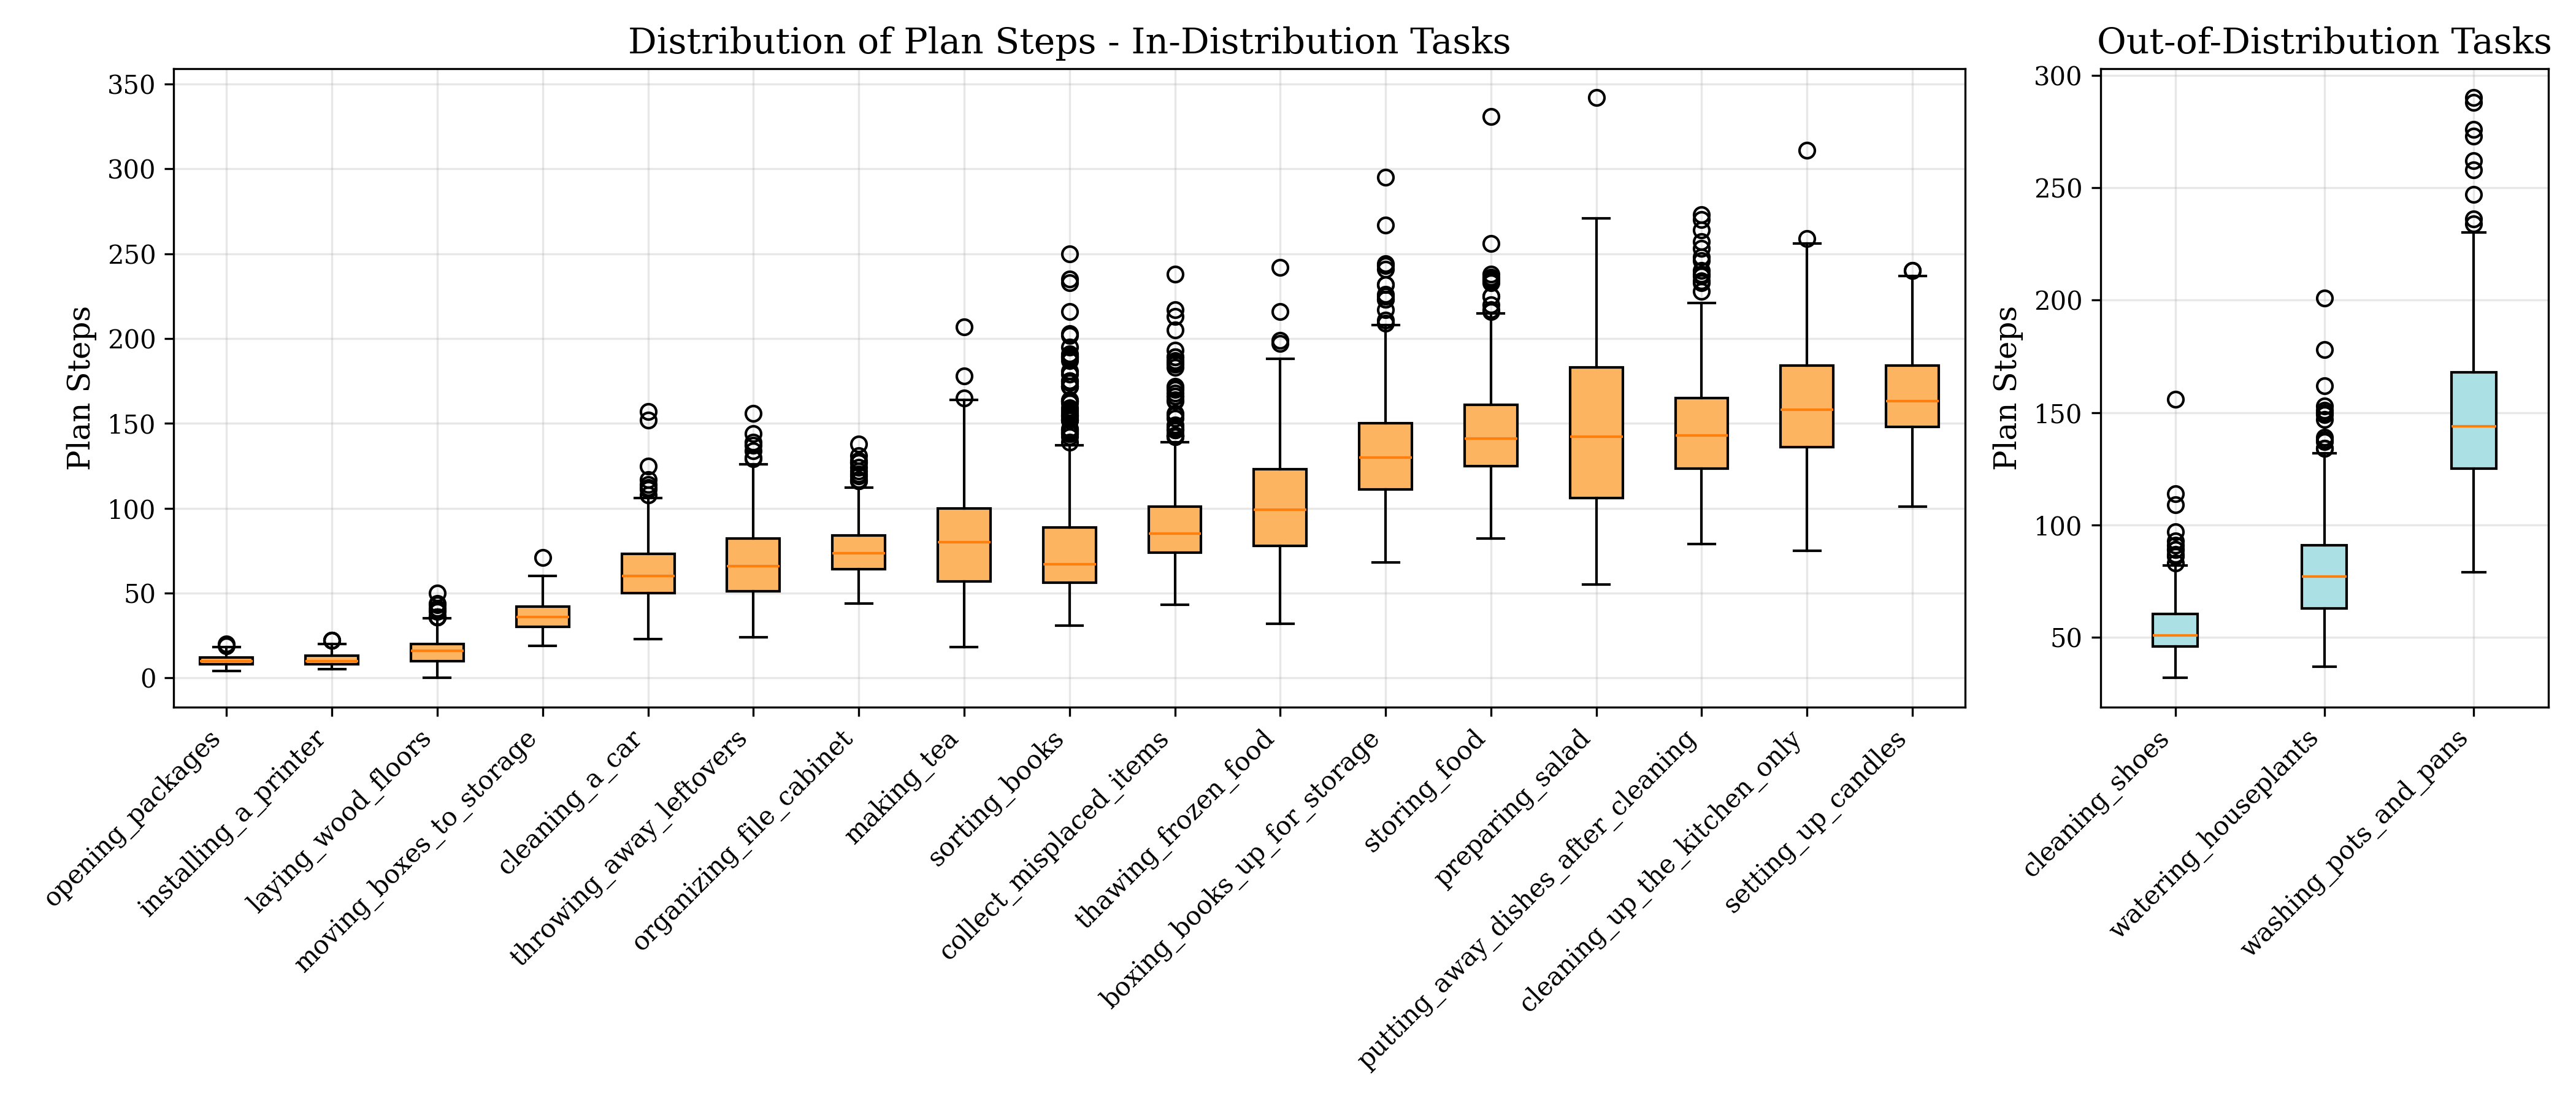
\includegraphics[width=\textwidth]{figures/plan_steps_distribution_boxplot.png}
    \caption{Distribution of reference plan steps required for tasks in \textsc{Mini-BEHAVIOR-Gran} obtained by \textsc{BWFS} classical planner.}
\end{figure*}


% ===== Fused Benchmark Task Spec Table (ID + OOD) with Goal Description =====

\begin{table*}[ht]
\small
\vspace{3mm}
\centering
\label{table:benchmark_task_spec}\scalebox{0.90}{{
\begin{tabular}{>{\centering\arraybackslash}p{4.9cm}||c|c|p{8.4cm}|c}
\toprule[0.4mm]
\cellcolor{mygray}\textbf{Task} & \cellcolor{mygray}\textbf{Split} & \cellcolor{mygray}\textbf{Class} & \cellcolor{mygray}\textbf{Goal Description} & \cellcolor{mygray}\textbf{Mean Steps} \\
\hline \hline
opening\_packages & ID & \cellcolor{green!20}\textbf{short} & Open every package. & 10.2 \\
installing\_a\_printer & ID & \cellcolor{green!20}\textbf{short} & Place a printer on a table and turn it on. & 10.6 \\
laying\_wood\_floors & ID & \cellcolor{green!20}\textbf{short} & Lay every plywood sheet on the floor, each touching at least one other sheet. & 15.9 \\
moving\_boxes\_to\_storage & ID & \cellcolor{green!20}\textbf{short} & Place every carton inside a shelf. & 36.3 \\
cleaning\_a\_car & ID & \cellcolor{green!20}\textbf{short} & Make at least one car dust-free. Place a rag and soap together inside a bucket. & 62.6 \\
throwing\_away\_leftovers & ID & \cellcolor{yellow!25}\textbf{middle} & Throw away every hamburger by placing it in a trash can. & 68.3 \\
organizing\_file\_cabinet & ID & \cellcolor{yellow!25}\textbf{middle} & Put a marker on a table and file every folder and document in a cabinet. & 75.5 \\
making\_tea & ID & \cellcolor{yellow!25}\textbf{middle} & Slice a lemon. Put a teapot on an activated stove. Keep a soaked teabag with the teapot. & 78.7 \\
sorting\_books & ID & \cellcolor{yellow!25}\textbf{middle} & Place every book and every hardback on a shelf. & 78.8 \\
collect\_misplaced\_items & ID & \cellcolor{yellow!25}\textbf{middle} & Place all gym shoes, necklaces, notebooks, and socks on a table. & 90.7 \\
thawing\_frozen\_food & ID & \cellcolor{yellow!25}\textbf{middle} & Place a date label next to a fish. Put every fish next to a sink. Set an olive next to a sink. & 101.7 \\
boxing\_books\_up\_for\_storage & ID & \cellcolor{blue!15}\textbf{long} & Place every book inside a box. & 134.4 \\
storing\_food & ID & \cellcolor{blue!15}\textbf{long} & Store every cookable item inside a cabinet. & 144.6 \\
preparing\_salad & ID & \cellcolor{blue!15}\textbf{long} & Slice all apples and tomatoes; place them on plates. Put every radish and lettuce on plates. Ensure each plate holds at least one cookable item. & 146.7 \\
putting\_away\_dishes\_after\_cleaning & ID & \cellcolor{blue!15}\textbf{long} & Put every plate inside a cabinet. & 147.7 \\
cleaning\_up\_the\_kitchen\_only & ID & \cellcolor{blue!15}\textbf{long} & Put every blender on a countertop. Refrigerate all apples and casseroles. Keep soap next to a sink. Make plates unstained and cabinets dust-free. Place each rag either beside or inside the sink. Store plates and vegetable oil in different cabinets. & 161.0 \\
setting\_up\_candles & ID & \cellcolor{blue!15}\textbf{long} & On every table, place three distinct candles on top. & 165.2 \\
\hline
cleaning\_shoes & OOD & \cellcolor{green!20}\textbf{short} & Leave a towel on the floor and make sure every shoe is unstained and dust-free. & 54.2 \\
watering\_houseplants & OOD & \cellcolor{yellow!25}\textbf{middle} & Water every potted plant until it is soaked. & 79.4 \\
washing\_pots\_and\_pans & OOD & \cellcolor{blue!15}\textbf{long} & Clean every teapot, kettle, and pan so they're unstained, then store each inside a cabinet. & 149.5 \\
\bottomrule[0.4mm]
\end{tabular}}}
\caption{Classification of tasks in \textsc{Mini-BEHAVIOR-Gran} based on the median number of plan steps, as determined by the \textsc{BWFS} planner. Tasks are categorized into short, middle, and long classes to reflect varying planning complexity based on plan length.}
\label{table:benchmark_class_based_on_plan_steps}
\end{table*}

Detailed statistics regarding the specific rule sets used for instruction generation and the resulting natural language statistics are discussed in the next section.


\section{Rule Set and Natural Language Prompt Examples For Different Tasks}
\label{app_sec:prompt_examples}

We present the rank 0 rule set for 10 over 20 household tasks in the Mini-BEHAVIOR-Gran environment. For other levels, please refer to the codebase at \url{mini-behavior-gran/mini_behavior/utils/policy_sketch/}. 

\subsection{Task 1: Laying Wood Floors}

\textbf{Features:}
\begin{itemize}[noitemsep]
    \item $H$: holding an isolated wood (plywood)
    \item $p$: distance to the nearest isolated wood
    \item $t$: distance to an arbitrary (non-held) wood we'll place next to
    \item $n$: number of isolated woods
\end{itemize}

\resizebox{\columnwidth}{!}{$
\begin{aligned}
\{\neg H, p>0, n >0\} &\mapsto \{p \downarrow, t?\} && \text{; move close to isolated wood} \\
\{\neg H, p=0, n >0\} &\mapsto \{H\} && \text{; pick up isolated wood when reachable} \\
\{H, t>0, n >0\} &\mapsto \{t\downarrow\} && \text{; move to some wood location} \\
\{H, n >0, t=0\} &\mapsto \{H?, n \downarrow, p?\} && \text{; drop the isolated wood next to other wood}
\end{aligned}
$}
\subsection{Task 2: Preparing Salad}

\textbf{Features:}
\begin{itemize}[noitemsep]
    \item $H_n$: holding a not-sliceable food
    \item $H_s$: holding a sliceable food
    \item $H_k$: holding a slicer
    \item $U$: number of sliceable food that is not sliced yet
    \item $d_p$: distance to the selected incomplete plate $p$
    \item $d_n, d_s$: distances to nearest not-sliceable / sliceable
    \item $k$: distance to a slicer (knife)
    \item $B$: selected plate $p$ complete bottom salad
    \item $n$: number of incomplete plates
    \item $nn$: number of plates that do not have bottom salad yet
\end{itemize}

\resizebox{\columnwidth}{!}{$
\noindent\textit{Acquire slicer:}
\begin{aligned}
\{U>0 , \neg H_k, k>0\} &\mapsto \{k \downarrow\} && \text{; move to slicer} \\
\{U>0 , \neg H_k, k=0\} &\mapsto \{H_k\} && \text{; hold a slicer} \\
\{U>0 , H_k, d_s > 0\} &\mapsto \{d_s \downarrow\} && \text{; move to sliceable food} \\
\{U>0 , H_k, d_s = 0\} &\mapsto \{U \downarrow, \neg H_k \} && \text{; cut sliceable food} \\
\{U=0 , H_k\} &\mapsto \{\neg H_k\} && \text{; put down slicer}
\end{aligned}
$}
\resizebox{\columnwidth}{!}{$
\noindent\textit{Place bottom salad:}
\begin{aligned}
\{n>0, U=0, nn>0, \neg B, \neg H_n, d_n>0\} &\mapsto \{d_n \downarrow\} \\
\{n>0, U=0,nn>0, \neg B, \neg H_n, d_n=0\} &\mapsto \{H_n\} \\
\{n>0, U=0,nn>0, \neg B, H_n, d_p>0\} &\mapsto \{d_p\downarrow\} \\
\{n>0, U=0, nn>0, \neg B, H_n, d_p=0\} &\mapsto \{B, nn \downarrow, \neg H_n\}
\end{aligned}
$}

\resizebox{\columnwidth}{!}{$
\noindent\textit{Handle sliceable salad:}
\begin{aligned}
\{nn=0, n>0, U=0 , \neg H_s, d_s>0\} &\mapsto \{d_s \downarrow\} && \text{; move to sliceable food} \\
\{nn=0, n>0, U=0 , \neg H_s, d_s=0\} &\mapsto \{H_s\} && \text{; pick up sliceable food} \\
\{nn=0, n>0, U=0 , H_s, d_p>0\} &\mapsto \{d_p \downarrow\} && \text{; move to the plate} \\
\{nn=0, n>0, U=0 , H_s, d_p=0\} &\mapsto \{n \downarrow, \neg H_s\} && \text{; put down sliced food}
\end{aligned}
$}

\subsection{Task 3: Cleaning Up the Kitchen Only}

\textbf{Features:}
\begin{itemize}[noitemsep]
    \item \textit{Holding flags:} $H_b$ (blender), $H_f$ (food), $H_s$ (soap), $H_r$ (rag), $H_p$ (plate), $H_o$ (vegetable oil)
    \item \textit{Distances:} $d_{ct}$ (countertop), $d_{fr}$ (fridge), $d_{si}$ (sink), $d_{c1}$ (cabinet for plate), $d_{c2}$ (cabinet for oil), $d_x$ (to object $x$)
    \item \textit{State booleans:} $\text{Open}(c)$, $\text{Tog}(s)$, $\text{Soaked}$, $\text{DustFree}(c)$, $\text{Clean}(p)$, $\text{OilIn}(c_2)$, $\text{Diff}$
    \item \textit{Counters:} $N_b$ (blenders not on countertop), $N_a$ (apples not in fridge), $N_{cas}$ (casseroles not in fridge), $N_s$ (soaps not next to sink), $N_{cab}$ (cabinets not dusted), $N_r$ (rags not next to sink), $N_{p\_clean}$ (plates not clean), $N_{oil}$ (oil not in cabinet), $N_{p\_store}$ (plates not stored), $N_{close}$ (closed furniture)
\end{itemize}

\resizebox{\columnwidth}{!}{$
\noindent\textit{Open Cabinet and Fridge:}
\begin{aligned}
\{N_{close} > 0, d_c>0\} &\mapsto \{d_c\downarrow\} && \text{; move toward closed furniture} \\
\{N_{close} > 0, d_c = 0\} &\mapsto \{N_{close}\downarrow\}
\end{aligned}
$}

\resizebox{\columnwidth}{!}{$
\noindent\textit{Oil placement:}
\begin{aligned}
\{N_{close} = 0,\neg H_o, d_{oil}>0\} &\mapsto \{d_{oil}\downarrow\} && \text{; approach oil} \\
\{N_{close} = 0,\neg H_o, d_{oil}=0\} &\mapsto \{H_o\} && \text{; pick up oil} \\
\{N_{close} = 0, H_o, N_{oil} > 0, d_{c2}>0\} &\mapsto \{d_{c2}\downarrow\} && \text{; go to cabinet } c_2 \\
\{N_{close} = 0, H_o, N_{oil} > 0, d_{c2} = 0\} &\mapsto \{N_{oil}\downarrow, \neg H_o\} && \text{; place oil in } c_2
\end{aligned}
$}

\resizebox{\columnwidth}{!}{$
\noindent\textit{Plate cleaning:}
\begin{aligned}
\{\neg \text{Tog}(s), d_{si}>0\} &\mapsto \{d_{si}\downarrow\} && \text{; toggle sink on} \\
\{\neg \text{Tog}(s), d_{si}=0\} &\mapsto \{\text{Tog}(s)\} \\
\{\neg H_r, d_{rag}>0\} &\mapsto \{d_{rag}\downarrow\} && \text{; get rag} \\
\{\neg H_r, d_{rag}=0\} &\mapsto \{H_r\} \\
\{H_r, \neg \text{Soaked}, d_{si}>0\} &\mapsto \{d_{si}\downarrow\} && \text{; soak rag} \\
\{H_r, \neg \text{Soaked}, d_{si}=0\} &\mapsto \{\text{Soaked}\} \\
\{H_r, \text{Soaked}, N_{p\_clean}>0, d_{plate}>0\} &\mapsto \{d_{plate}\downarrow\} \\
\{H_r, \text{Soaked}, N_{p\_clean}>0, d_{plate}=0\} &\mapsto \{N_{p\_clean}\downarrow, d_{plate}?\}
\end{aligned}
$}
\resizebox{\columnwidth}{!}{$
\noindent\textit{Plate placement distinct from oil:}
\begin{aligned}
\{N_{close} =0 , N_{oil}=0, N_{p\_clean} =0 ,\neg H_p, N_{p\_store}>0, d_{plate}>0\} &\mapsto \{d_{plate}\downarrow\} \\
\{N_{close} =0 , N_{oil}=0, N_{p\_clean} =0 , \neg H_p, N_{p\_store}>0, d_{plate}=0\} &\mapsto \{H_p\} \\
\{N_{close} =0 , N_{oil}=0, N_{p\_clean} =0 , H_p, N_{p\_store}>0, d_{c1}>0\} &\mapsto \{d_{c1}\downarrow\} \\
\{N_{close} =0 , N_{oil}=0, N_{p\_clean} =0 , H_p, N_{p\_store}>0, d_{c1}=0\} &\mapsto \{N_{p\_store}\downarrow, \neg H_p\}
\end{aligned}
$}

\resizebox{\columnwidth}{!}{$
\noindent\textit{Blender to countertop:}
\begin{aligned}
\{N_b > 0, \neg H_b, d_{blender}>0\} &\mapsto \{d_{blender}\downarrow\} \\
\{N_b > 0, \neg H_b, d_{blender}=0\} &\mapsto \{H_b\} \\
\{H_b, N_b>0, d_{ct}>0\} &\mapsto \{d_{ct}\downarrow\} \\
\{H_b, N_b>0, d_{ct}=0\} &\mapsto \{N_b\downarrow, \neg H_b\}
\end{aligned}
$}

\resizebox{\columnwidth}{!}{$
\noindent\textit{Apple to fridge:}
\begin{aligned}
\{N_{close} =0,\neg H_f, d_{apple}>0\} &\mapsto \{d_{apple}\downarrow\} \\
\{N_{close} =0,\neg H_f, d_{apple}=0\} &\mapsto \{H_f\} \\
\{N_{close} =0,H_f, N_a>0, d_{fr}>0\} &\mapsto \{d_{fr}\downarrow\} \\
\{N_{close} =0,H_f, N_a>0, d_{fr}=0\} &\mapsto \{N_a\downarrow, \neg H_f\}
\end{aligned}
$}

\resizebox{\columnwidth}{!}{$
\noindent\textit{Casserole to fridge:}
\begin{aligned}
\{N_{close} =0 ,\neg H_f, d_{casserole}>0\} &\mapsto \{d_{casserole}\downarrow\} \\
\{N_{close} =0 ,\neg H_f, d_{casserole}=0\} &\mapsto \{H_f\} \\
\{N_{close} =0 ,H_f, N_{cas}>0, d_{fr}>0\} &\mapsto \{d_{fr}\downarrow\} \\
\{N_{close} =0 ,H_f, N_{cas}>0, d_{fr}=0\} &\mapsto \{N_{cas}\downarrow, \neg H_f\}
\end{aligned}
$}

\resizebox{\columnwidth}{!}{$
\noindent\textit{Cabinet dusting:}
\begin{aligned}
\{\neg H_r, d_{rag}>0\} &\mapsto \{d_{rag}\downarrow\} && \text{; get rag} \\
\{\neg H_r, d_{rag}=0\} &\mapsto \{H_r\} \\
\{H_r, N_{cab}>0, d_c>0\} &\mapsto \{d_c\downarrow\} && \text{; clean cabinet} \\
\{H_r, N_{cab}>0, d_c=0\} &\mapsto \{N_{cab}\downarrow, \neg H_r\}
\end{aligned}
$}

\resizebox{\columnwidth}{!}{$
\noindent\textit{Rag near/inside sink:}
\begin{aligned}
\{N_{cab} = 0, N_{p\_clean} = 0,\neg H_r, d_{rag}>0\} &\mapsto \{d_{rag}\downarrow\} \\
\{N_{cab} = 0, N_{p\_clean} = 0,\neg H_r, d_{rag}=0\} &\mapsto \{H_r\} \\
\{N_{cab} = 0, N_{p\_clean} = 0,H_r, N_r>0, d_{si}>0\} &\mapsto \{d_{si}\downarrow\} \\
\{N_{cab} = 0, N_{p\_clean} = 0,H_r, N_r>0, d_{si}=0\} &\mapsto \{N_r\downarrow, \neg H_r\}
\end{aligned}
$}

\resizebox{\columnwidth}{!}{$
\noindent\textit{Soap next to sink:}
\begin{aligned}
\{N_{cab} = 0, N_{p\_clean} = 0,\neg H_s, d_{soap}>0\} &\mapsto \{d_{soap}\downarrow\} \\
\{N_{cab} = 0, N_{p\_clean} = 0,\neg H_s, d_{soap}=0\} &\mapsto \{H_s\} \\
\{N_{cab} = 0, N_{p\_clean} = 0,H_s, N_s>0, d_{si}>0\} &\mapsto \{d_{si}\downarrow\} \\
\{N_{cab} = 0, N_{p\_clean} = 0,H_s, N_s>0, d_{si}=0\} &\mapsto \{N_s\downarrow, \neg H_s\}
\end{aligned}
$}

\subsection{Task 4: Organizing File Cabinet}

\textbf{Features:}
\begin{itemize}[noitemsep]
    \item $H_m$: holding a marker
    \item $H_f$: holding a folder
    \item $H_d$: holding a document
    \item $p_m$: distance to the nearest marker
    \item $p_f$: distance to the nearest folder
    \item $p_d$: distance to the nearest document
    \item $p_t$: distance to a table
    \item $p_c$: distance to a valid cabinet target
    \item $N_m$: number of markers not on a table
    \item $N_f$: number of folders not in a cabinet
    \item $N_d$: number of documents not in a cabinet
    \item $N_o$: number of closed cabinets
\end{itemize}

\resizebox{\columnwidth}{!}{$
\noindent\textit{Opening Cabinet:}
\begin{aligned}
\{N_o > 0, p_c > 0\} &\mapsto \{p_c \downarrow\} && \text{; move toward a closed cabinet} \\
\{N_o > 0, p_c = 0\} &\mapsto \{N_o \downarrow\} && \text{; open the cabinet when reachable}
\end{aligned}
$}
\resizebox{\columnwidth}{!}{$
\noindent\textit{Marker task:}
\begin{aligned}
\{N_m > 0, \neg H_m, p_m > 0\} &\mapsto \{p_m \downarrow, p_t ?\} && \text{; move toward the nearest marker} \\
\{N_m > 0, \neg H_m, p_m = 0\} &\mapsto \{H_m, p_t ?\} && \text{; pick up the marker when reachable} \\
\{N_m > 0, H_m, p_t > 0\} &\mapsto \{p_t \downarrow\} && \text{; move toward a table} \\
\{N_m > 0, H_m, p_t = 0\} &\mapsto \{N_m \downarrow, \neg H_m, p_m ?\} && \text{; put marker on table}
\end{aligned}
$}
\resizebox{\columnwidth}{!}{$
\noindent\textit{Folder task:}
\begin{aligned}
\{N_f > 0, N_o = 0, \neg H_f, p_f > 0\} &\mapsto \{p_f \downarrow, p_c ?\} \\
\{N_f > 0, N_o = 0, \neg H_f, p_f = 0\} &\mapsto \{H_f, p_c ?\} \\
\{N_f > 0, N_o = 0, H_f, p_c > 0\} &\mapsto \{p_c \downarrow\} \\
\{N_f > 0, N_o = 0, H_f, p_c = 0\} &\mapsto \{N_f \downarrow, \neg H_f, p_f ?\}
\end{aligned}
$}
\resizebox{\columnwidth}{!}{$
\noindent\textit{Document task:}
\begin{aligned}
\{N_d > 0, N_o = 0, \neg H_d, p_d > 0\} &\mapsto \{p_d \downarrow, p_c ?\} \\
\{N_d > 0, N_o = 0, \neg H_d, p_d = 0\} &\mapsto \{H_d, p_c ?\} \\
\{N_d > 0, N_o = 0, H_d, p_c > 0\} &\mapsto \{p_c \downarrow\} \\
\{N_d > 0, N_o = 0, H_d, p_c = 0\} &\mapsto \{N_d \downarrow, \neg H_d, p_d ?\}
\end{aligned}
$}

\subsection{Task 5: Thawing Frozen Food}

\textbf{Features:}
\begin{itemize}[noitemsep]
    \item $H_{fish}$: holding a fish
    \item $H_{olive}$: holding an olive
    \item $H_{date}$: holding a date
    \item $p_{fish}$: distance to the nearest fish
    \item $p_{olive}$: distance to the nearest olive
    \item $p_{date}$: distance to the nearest date
    \item $p_{sink}$: distance to a sink
    \item $N_{fish}$: number of fish not next to a sink
    \item $N_{olive}$: number of olives not next to a sink
    \item $N_{date}$: number of dates not next to a fish
\end{itemize}

\resizebox{\columnwidth}{!}{$
\noindent\textit{Fish Task:}
\begin{aligned}
\{\neg H_{fish}, p_{fish} > 0\} &\mapsto \{p_{fish} \downarrow\} \\
\{\neg H_{fish}, p_{fish} = 0\} &\mapsto \{H_{fish}\} \\
\{H_{fish}, p_{sink} > 0\} &\mapsto \{p_{sink} \downarrow\} \\
\{H_{fish}, p_{sink} = 0\} &\mapsto \{N_{fish} \downarrow, \neg H_{fish}, p_{fish} ?\}
\end{aligned}
$}

\resizebox{\columnwidth}{!}{$
\noindent\textit{Olive Task:}
\begin{aligned}
\{\neg H_{olive}, p_{olive} > 0\} &\mapsto \{p_{olive} \downarrow\} \\
\{\neg H_{olive}, p_{olive} = 0\} &\mapsto \{H_{olive}\} \\
\{H_{olive}, p_{sink} > 0\} &\mapsto \{p_{sink} \downarrow\} \\
\{H_{olive}, p_{sink} = 0\} &\mapsto \{N_{olive} \downarrow, \neg H_{olive}, p_{olive} ?\}
\end{aligned}
$}

\resizebox{\columnwidth}{!}{$
\noindent\textit{Date Task:}
\begin{aligned}
\{\neg H_{date}, N_{\text{fish olive}}= 0, p_{date} > 0\} &\mapsto \{p_{date} \downarrow\} \\
\{\neg H_{date}, N_{\text{fish olive}}= 0,p_{date} = 0\} &\mapsto \{H_{date}\} \\
\{H_{date}, N_{\text{fish olive}}= 0,p_{fish} > 0\} &\mapsto \{p_{fish} \downarrow\} \\
\{H_{date}, N_{\text{fish olive}}= 0, p_{fish} = 0\} &\mapsto \{N_{date} \downarrow, \neg H_{date}, p_{date} ?\}
\end{aligned}
$}


\subsection{Task 6: Making Tea}

\textbf{Features:}
\begin{itemize}[noitemsep]
    \item $H_l$: holding a lemon
    \item $H_{knife}$: holding a knife
    \item $H_t$: holding a teapot
    \item $H_{tb}$: holding a tea bag
    \item $p_l$: distance to the nearest lemon
    \item $p_{knife}$: distance to the knife
    \item $p_t$: distance to the nearest teapot
    \item $p_{tb}$: distance to the nearest tea bag
    \item $p_s$: distance to the stove
    \item $p_{sink}$: distance to the sink
    \item $\text{is\_sliced}(\text{lemon})$: whether the lemon is sliced
    \item $\text{is\_toggled}(\text{stove})$: whether the stove is toggled on
    \item $\text{is\_toggled}(\text{sink})$: whether the sink is toggled on
    \item $\text{is\_soaked}(\text{tea\_bag})$: whether the tea bag is soaked
    \item $\text{atsamelocation}(\text{tea\_bag}, \text{teapot})$: tea bag at same location as teapot
    \item $\text{onTop}(\text{teapot}, \text{stove})$: teapot on stove
\end{itemize}

\resizebox{\columnwidth}{!}{$
\noindent\textit{Toggle stove:}
\begin{aligned}
\{\neg \text{is\_toggled}(\text{stove}), p_s > 0\} &\mapsto \{p_s \downarrow\} \\
\{\neg \text{is\_toggled}(\text{stove}), p_s = 0\} &\mapsto \{\text{is\_toggled}(\text{stove})\}
\end{aligned}
$}
\resizebox{\columnwidth}{!}{$
\noindent\textit{Slice lemon:}
\begin{aligned}
\{\neg H_{knife}, p_{knife} > 0, \neg \text{is\_sliced}(\text{lemon})\} &\mapsto \{p_{knife} \downarrow\} \\
\{\neg H_{knife}, p_{knife} = 0, \neg \text{is\_sliced}(\text{lemon})\} &\mapsto \{H_{knife}\} \\
\{H_{knife}, \neg \text{is\_sliced}(\text{lemon}), p_{l} > 0\} &\mapsto \{p_{l} \downarrow\} \\
\{H_{knife}, \neg \text{is\_sliced}(\text{lemon}), p_{l} = 0\} &\mapsto \{\text{is\_sliced}(\text{lemon})\} \\
\{H_{knife}, \text{is\_sliced}(\text{lemon})\} &\mapsto \{\neg H_{knife}, p_{knife} ?\}
\end{aligned}
$}
\resizebox{\columnwidth}{!}{$
\noindent\textit{Handle teapot:}
\begin{aligned}
\{\neg \text{atsameloc}(\text{tb}, \text{tp}), \neg \text{onTop}(\text{tp}, \text{st}), \neg H_t, p_t > 0\} &\mapsto \{p_t \downarrow\} \\
\{\neg \text{atsameloc}(\text{tb}, \text{tp}), \neg \text{onTop}(\text{tp}, \text{st}), \neg H_t, p_t = 0\} &\mapsto \{H_t\} \\
\{\neg \text{atsameloc}(\text{tb}, \text{tp}), \neg \text{onTop}(\text{tp}, \text{st}), H_t, p_s > 0\} &\mapsto \{p_s \downarrow\} \\
\{\neg \text{atsameloc}(\text{tb}, \text{tp}), \neg \text{onTop}(\text{tp}, \text{st}), H_t, p_s = 0\} &\mapsto \{\text{onTop}(\text{tp}, \text{st}), \neg H_t, p_t ?\} \\
\{\neg \text{atsameloc}(\text{tb}, \text{tp}), \text{onTop}(\text{tp}, \text{st}), \neg H_{tb}, p_{tb} > 0\} &\mapsto \{p_{tb} \downarrow\} \\
\{\neg \text{atsameloc}(\text{tb}, \text{tp}), \text{onTop}(\text{tp}, \text{st}), \neg H_{tb}, p_{tb} = 0\} &\mapsto \{H_{tb}\} \\
\{\neg \text{atsameloc}(\text{tb}, \text{tp}), \text{onTop}(\text{tp}, \text{st}), H_{tb}, p_t > 0\} &\mapsto \{p_t \downarrow\} \\
\{H_{tb}, \neg \text{atsameloc}(\text{tb}, \text{tp}), \text{onTop}(\text{tp}, \text{st}), p_t = 0\} &\mapsto \{\text{atsameloc}(\text{tb}, \text{tp}), \neg H_{tb}, p_{tb} ?\}
\end{aligned}
$}

\subsection{Task 7: Opening Packages}

\textbf{Features:}
\begin{itemize}[noitemsep]
    \item $p$: distance to the nearest package
    \item $N$: number of unopened packages
\end{itemize}

\resizebox{\columnwidth}{!}{$
\begin{aligned}
\{N > 0, p > 0\} &\mapsto \{p \downarrow\} && \text{; move toward the nearest unopened package} \\
\{N > 0, p = 0\} &\mapsto \{N \downarrow\} && \text{; open the package when reachable}
\end{aligned}
$}

\subsection{Task 8: Boxing Books Up for Storage}

\textbf{Features:}
\begin{itemize}[noitemsep]
    \item $H$: holding an unboxed book
    \item $p$: distance to the nearest unboxed book
    \item $b$: distance to a valid box target
    \item $N$: number of unboxed books
\end{itemize}

\resizebox{\columnwidth}{!}{$
\begin{aligned}
\{\neg H, p > 0\} &\mapsto \{p \downarrow, b ?\} && \text{; move toward the nearest unboxed book} \\
\{\neg H, p = 0\} &\mapsto \{H\} && \text{; pick up the book when reachable} \\
\{H, N > 0, b > 0\} &\mapsto \{b \downarrow\} && \text{; move toward a chosen box spot} \\
\{H, N > 0, b = 0\} &\mapsto \{\neg H, N \downarrow, p ?\} && \text{; place the book into the box}
\end{aligned}
$}

\subsection{Task 9: Collect Misplaced Items}

\textbf{Features:}
\begin{itemize}[noitemsep]
    \item $H_s$: holding a gym shoe
    \item $H_n$: holding a necklace
    \item $H_b$: holding a notebook
    \item $H_k$: holding a sock
    \item $p_s$: distance to the nearest gym shoe
    \item $p_n$: distance to the nearest necklace
    \item $p_b$: distance to the nearest notebook
    \item $p_k$: distance to the nearest sock
    \item $p_t$: distance to a table
    \item $N_s$: number of gym shoes not on a table
    \item $N_n$: number of necklaces not on a table
    \item $N_b$: number of notebooks not on a table
    \item $N_k$: number of socks not on a table
\end{itemize}

\resizebox{\columnwidth}{!}{$
\noindent\textit{Gym shoe task:}
\begin{aligned}
\{\neg H_s, N_s > 0, p_s > 0\} &\mapsto \{p_s \downarrow, p_t ?\} \\
\{\neg H_s, N_s > 0, p_s = 0\} &\mapsto \{H_s, p_t ?\} \\
\{H_s, N_s > 0, p_t > 0\} &\mapsto \{p_t \downarrow\} \\
\{H_s, N_s > 0, p_t = 0\} &\mapsto \{N_s \downarrow, \neg H_s, p_s ?\}
\end{aligned}
$}
\resizebox{\columnwidth}{!}{$
\noindent\textit{Necklace task:}
\begin{aligned}
\{\neg H_n, N_n > 0, p_n > 0\} &\mapsto \{p_n \downarrow, p_t ?\} \\
\{\neg H_n, N_n > 0, p_n = 0\} &\mapsto \{H_n, p_t ?\} \\
\{H_n, N_n > 0, p_t > 0\} &\mapsto \{p_t \downarrow\} \\
\{H_n, N_n > 0, p_t = 0\} &\mapsto \{N_n \downarrow, \neg H_n, p_n ?\}
\end{aligned}
$}
\resizebox{\columnwidth}{!}{$
\noindent\textit{Notebook task:}
\begin{aligned}
\{\neg H_b, N_b > 0, p_b > 0\} &\mapsto \{p_b \downarrow, p_t ?\} \\
\{\neg H_b, N_b > 0, p_b = 0\} &\mapsto \{H_b, p_t ?\} \\
\{H_b, N_b > 0, p_t > 0\} &\mapsto \{p_t \downarrow\} \\
\{H_b, N_b > 0, p_t = 0\} &\mapsto \{N_b \downarrow, \neg H_b, p_b ?\}
\end{aligned}
$}
\resizebox{\columnwidth}{!}{$
\noindent\textit{Sock task:}
\begin{aligned}
\{\neg H_k, N_k > 0, p_k > 0\} &\mapsto \{p_k \downarrow, p_t ?\} \\
\{\neg H_k, N_k > 0, p_k = 0\} &\mapsto \{H_k, p_t ?\} \\
\{H_k, N_k > 0, p_t > 0\} &\mapsto \{p_t \downarrow\} \\
\{H_k, N_k > 0, p_t = 0\} &\mapsto \{N_k \downarrow, \neg H_k, p_k ?\}
\end{aligned}
$}

\subsection{Task 10: Putting Away Dishes After Cleaning}

\textbf{Features:}
\begin{itemize}[noitemsep]
    \item $H$: holding a plate
    \item $p$: distance to the nearest plate
    \item $b$: distance to a valid cabinet target
    \item $N$: number of unboxed plates
    \item $\text{is\_opened}$: whether the cabinet is opened
\end{itemize}

\resizebox{\columnwidth}{!}{$
\begin{aligned}
\{\neg \text{is\_opened}, b > 0\} &\mapsto \{b \downarrow\} && \text{; move toward the cabinet} \\
\{\neg \text{is\_opened}, b = 0\} &\mapsto \{\text{is\_opened}\} && \text{; open the cabinet when reachable} \\
\{\neg H, N > 0, p > 0, \text{is\_opened}\} &\mapsto \{p \downarrow, b ?\} \\
\{\neg H, N > 0, p = 0, \text{is\_opened}\} &\mapsto \{H, b ?\} \\
\{H, N > 0, b > 0, \text{is\_opened}\} &\mapsto \{b \downarrow\} \\
\{H, N > 0, b = 0, \text{is\_opened}\} &\mapsto \{\neg H, N \downarrow, p ?\}
\end{aligned}
$}



\subsection{Instruction Generation Statistics} We used a template-based generator to translate the symbolic rule sets into natural language instructions, ensuring alignment with the VLA's training data format. Table \ref{tab:instruction_stats} presents the summary statistics for the generated instructions across the three granularity levels.

\begin{table*}[t] 
\centering 
\caption{Statistics of generated natural language instructions across granularity levels.} 
\label{tab:instruction_stats} 
\resizebox{\textwidth}{!}{% 
\begin{tabular}{l|c|c|c|c|c|c|c|c}
\toprule 
\textbf{Granularity} & \textbf{Count} & \textbf{Avg Length} & \textbf{Std Length} & \textbf{Min} & \textbf{Max} & \textbf{Unique Tokens} & \textbf{TTR} & \textbf{Avg Sent. Length} \\ 
 & & \textbf{(words)} & & & & & \textbf{(Type-Token Ratio)} & \\ 
\midrule
\textbf{Fine (F)} & 1636 & 41.12 & 11.36 & 19 & 87 & 140 & 0.0021 & 41.12 \\ 
\textbf{Medium (M)} & 859 & 38.62 & 12.76 & 22 & 81 & 108 & 0.0033 & 38.62 \\ 
\textbf{Coarse (C)} & 587 & 33.60 & 13.39 & 22 & 95 & 94 & 0.0048 & 33.60 \\ 
\bottomrule 
\end{tabular}% 
} 
\end{table*}



\section{Implementation Details}
\label{app_sec:implementation_details}

\subsection{Model Architecture}

Our policy is built upon the OpenVLA architecture \citep{DBLP:conf/corl/KimPKXB0RFSVKBT24}. Specifically, we utilize the Prismatic-7B backbone \citep{DBLP:conf/icml/Karamcheti0BLKS24}, which integrates a frozen Llama-2-7B language model with fused visual features. The visual encoder consists of a dual-stream setup combining SigLIP (for semantic understanding) and DINOv2 (for fine-grained spatial geometry) \citep{DBLP:conf/iccv/ZhaiM0B23,DBLP:journals/tmlr/OquabDMVSKFHMEA24}.

\subsection{Training Configuration}

We fine-tune the model using Low-Rank Adaptation (LoRA) on the language model backbone, keeping the visual encoders frozen. All training setting variants (Pure, Centroid, Axial) share the same underlying training hyperparameters to ensure fair comparison.

Hardware and Duration: Training was conducted on a single node equipped with 8$\times$ NVIDIA A100 GPUs. A standard training run for 100,000 steps took approximately 23 hours to complete.

Table \ref{tab:hyperparameters} summarizes the core hyperparameters used across our experiments.

\begin{table}[H]
\centering
\caption{Hyperparameters for OpenVLA fine-tuning on \textsc{Mini-BEHAVIOR-Gran}.}
\label{tab:hyperparameters}
\resizebox{\columnwidth}{!}{%
\begin{tabular}{l|c}
\toprule
\textbf{Hyperparameter} & \textbf{Value} \\
\midrule
Base Model & Prismatic-7B (Llama-2) \\
Visual Encoders & SigLIP + DINOv2 \\
Parameter Efficient Tuning & LoRA (Rank $r=32$) \\
Compute Hardware & 8$\times$ NVIDIA A100 \\
Training Duration & $\sim$23 hours \\
Optimization Steps & 100,000 \\
Steps Before Decay & 80,000 \\
Learning Rate & $2.5 \times 10^{-4}$ \\
Batch Size (per GPU) & $7 - 8$ \\
\bottomrule
\end{tabular} %
}
\end{table}

We also train a lightweight VLM predictor to quantify instruction predictability via perplexity. The model is fine-tuned using Low-Rank Adaptation (LoRA) on the Qwen3-VL-4B-Instruct backbone, with vision encoders frozen to preserve visual grounding capabilities established during pretraining. All models are trained on \textsc{Mini-BEHAVIOR-Gran} instruction and image training data pairs, with training and evaluation splits maintained consistently across experiments. Hardware and Duration: Training was conducted on a single node equipped with 4$\times$ NVIDIA RTX 5090 GPUs. Each training run for 2 epochs. Table \ref{tab:qwen_hyperparameters} summarizes the core hyperparameters used for VLM predictor training.

\begin{table}[H]
\centering
\caption{Hyperparameters for Qwen3-VL-4B-Instruct fine-tuning on \textsc{Mini-BEHAVIOR-Gran} (High-domain).}
\label{tab:qwen_hyperparameters}
\resizebox{\columnwidth}{!}{%
\begin{tabular}{l|c}
\toprule
\textbf{Hyperparameter} & \textbf{Value} \\
\midrule
Base Model & Qwen3-VL-4B-Instruct \\
Visual Encoders & Frozen (Qwen3-VL native) \\
Parameter Efficient Tuning & LoRA (Rank $r=64$, $\alpha=128$) \\
LoRA Target Modules & All linear layers \\
Compute Hardware & 4$\times$ NVIDIA RTX 5090 \\
Training Epochs & 2 \\
Learning Rate & $1.0 \times 10^{-5}$ \\
Learning Rate Scheduler & Cosine with 10\% warmup \\
Batch Size (per GPU) & 32 \\
Seed & [42,50,60] \\
Gradient Accumulation Steps & 1 \\
DeepSpeed Strategy & Zero-2 \\
\bottomrule
\end{tabular} %
}
\end{table}



\section{Additional Experimental Results}
\label{app_sec:additional_experimental_results}

This section provides additional detailed per-task performance breakdowns, and failure mode distributions.

\subsection{Detailed Task Performance} 

Figure \ref{fig:per_task_success_rate} details the success rates across all 20 tasks in the benchmark. We see some tasks are too difficult to solve and thus low across all instruction granularity. And then we also see the U shape trends in most tasks, showing the same phenomenon we discussed in \textbf{(Q1)} that both very fine and very coarse instructions are easier for VLA to follow.


\begin{figure*}[t]
    \centering
    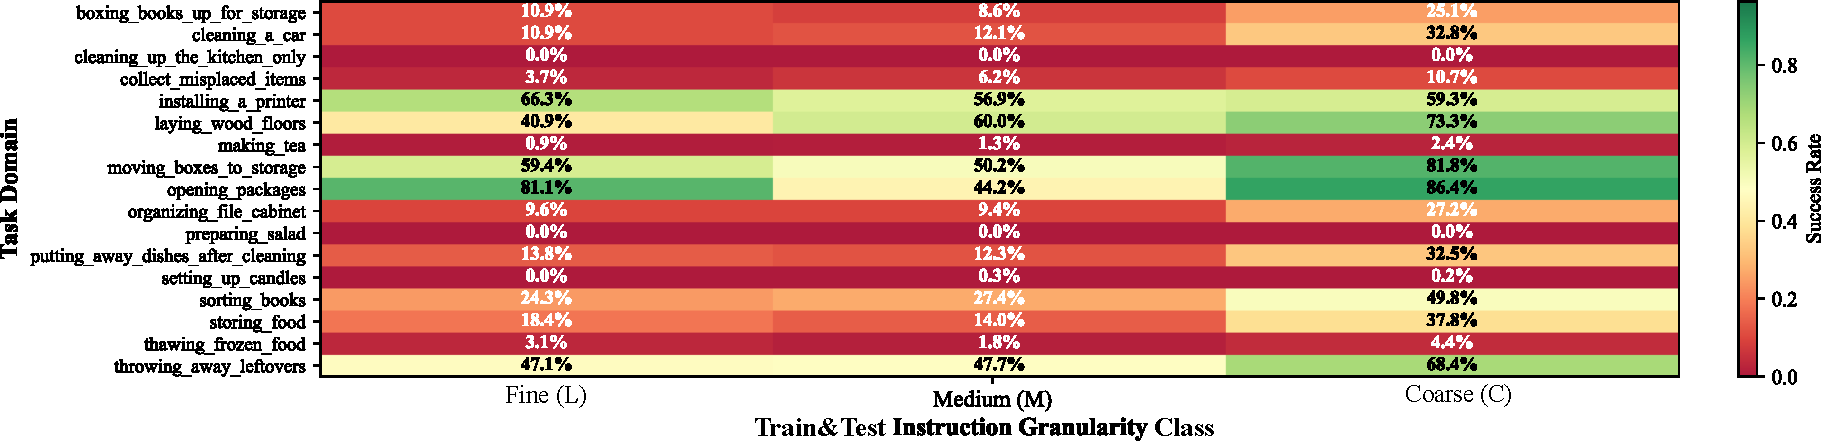
\includegraphics[width=\linewidth]{figures/q1_task_success_rate.pdf}
    \caption{Detailed per-task success rates.}
    \label{fig:per_task_success_rate}
\end{figure*}

\subsection{Detailed Attention Analysis Table}
\label{app_sec:full_attention_analysis_table}

We quantify the internal information-gathering behavior of Vision-Language-Action (VLA) models by analyzing the \textbf{attention weight distribution of the action tokens}. In these architectures, the action tokens serve as the terminal query point; their attention allocation reveals which input modalities (vision vs. language) the model prioritizes at different stages of its internal processing hierarchy.

\subsubsection{Input Sequence Formalization}
The input sequence $\mathcal{S}$ is composed of visual patches, linguistic tokens, and action tokens. Given a single sample, the sequence layout is defined as:
\begin{equation}
    \mathcal{S} = [ \texttt{BOS}, \underbrace{v_1, \dots, v_P}_{\text{vision}}, \underbrace{t_1, \dots, t_T}_{\text{text}}, \underbrace{a_1, \dots, a_A}_{\text{action}}, \texttt{EOS} ]
\end{equation}
where $P$ is the number of visual patch tokens, $T$ is the number of text tokens (comprising both prompt prefix and task instruction), and $A$ is the number of action tokens (where $A = d_{\text{action}} \times \text{chunk size}$). 

For analysis, we exclude the $[\texttt{BOS}]$ and $[\texttt{EOS}]$ boundary tokens. For each layer $\ell \in \{1, \dots, L\}$, we extract the trimmed attention tensor:
\begin{equation}
    \mathbf{A}^{(\ell)} \in \mathrm{R}^{H \times (P+T+A) \times (P+T+A)}
\end{equation}

\subsubsection{Partitioning of Semantic Regions}
To distinguish between general linguistic context and specific task instructions, we partition the key dimension (columns) of $\mathbf{A}^{(\ell)}$ into four non-overlapping semantic regions:

\textit{Note: For models utilizing compressed instruction patches, the compressed embeddings are mapped to the Dynamic Text category to ensure functional consistency across architectures.}

\subsubsection{Quantitative Measurement}
For each layer $\ell$ and head $h$, we isolate the \textbf{action-to-key} sub-matrix $\mathbf{A}^{(\ell)}_{h,\text{action} \to \text{key}} \in \mathrm{R}^{A \times (P+T+A)}$. The mean attention mass allocated to a specific region $R = [r_{\text{start}}, r_{\text{end}})$ is computed by summing weights across the region and averaging over the $A$ action tokens:
\begin{equation}
    \text{attn}_h(R) = \frac{1}{A} \sum_{i=1}^{A} \sum_{j=r_{\text{start}}}^{r_{\text{end}}-1} \mathbf{A}^{(\ell)}_{h,\text{action} \to \text{key}}[i, j]
\end{equation}

\subsubsection{Aggregation and Normalization}
To derive a layer-wise modality reliance score, we perform the following:
\begin{enumerate}
    \item \textbf{Head Averaging}: $\text{attn}(R) = \frac{1}{H} \sum_{h=1}^{H} \text{attn}_h(R)$.
    \item \textbf{Sample Mean}: Values are averaged across all samples within a specific granularity-model pair.
    \item \textbf{Simplex Normalization}: The final regional shares $\hat{a}_R$ are normalized such that $\sum_{R} \hat{a}_R = 1$.
\end{enumerate}

\subsubsection{Statistical Trend Hypothesis Testing}
We define three binary indicators to test the \textbf{Shallow Grounding Hypothesis} layer-wise:
\begin{itemize}
    \item \textbf{T1 (Lang $\uparrow$)}: $\hat{a}_{\text{text}}(\text{Medium}) > \hat{a}_{\text{text}}(\text{Fine})$
    \item \textbf{T2 (Lang $\downarrow$)}: $\hat{a}_{\text{text}}(\text{Medium}) > \hat{a}_{\text{text}}(\text{Coarse})$
    \item \textbf{T3 (Vis $\uparrow$)}: $\hat{a}_{\text{vis}}(\text{Coarse}) > \hat{a}_{\text{vis}}(\text{Medium})$
\end{itemize}
We assess the significance of these trends across $N=32$ layers using a \textbf{one-sided Binomial test} ($H_0: p=0.5$). Significance is reported as $^{*}p < 0.05$ and $^{**}p < 0.01$. Confidence intervals for proportions are calculated using the \textbf{Clopper-Pearson} method. The full statistical breakdown is presented in \Cref{tab:full_stats_appendix}.

\begin{table*}[h]
\centering
\small
\begin{tabular}{ll cccc c}
\toprule
\textbf{Model} & \textbf{Trend} & \textbf{k/N} & \textbf{Prop.} & \textbf{95\% CI} & \textbf{$H_0$} & \textbf{$p$-value} \\
\midrule
Autoregressive     & T1 & 25/32 & 78.1\% & [0.600, 0.907] & 50.0\% & 0.0011 \\
                   & T2 & 4/32  & 12.5\% & [0.035, 0.290] & 50.0\% & 1.0000 \\
                   & T3 & 21/32 & 65.6\% & [0.468, 0.814] & 50.0\% & 0.1102 \\
\midrule
Parallel Decoding  & T1 & 5/32  & 15.6\% & [0.053, 0.328] & 50.0\% & 1.0000 \\
                   & T2 & 9/32  & 28.1\% & [0.137, 0.467] & 50.0\% & 0.9965 \\
                   & T3 & 5/32  & 15.6\% & [0.053, 0.328] & 50.0\% & 1.0000 \\
\midrule
Discrete Diffusion & T1 & 17/32 & 53.1\% & [0.347, 0.709] & 50.0\% & 0.4300 \\
                   & T2 & 23/32 & 71.9\% & [0.533, 0.863] & 50.0\% & 0.0100 \\
                   & T3 & 24/32 & 75.0\% & [0.566, 0.885] & 50.0\% & 0.0035 \\
\bottomrule
\end{tabular}
\caption{Detailed statistical analysis of layer-wise attention trends across architectures. P-values are calculated using a one-sided Binomial test against a null hypothesis ($H_0$) of 0.5. Confidence intervals (CI) are calculated at the 95\% level.}
\label{tab:full_stats_appendix}
\end{table*}

\subsection{Failure Analysis} 
Figure \ref{fig:failure_type_dist_by_width} presents the distribution of failure types across varying instruction widths. It confirms that low width encounters regression failures more frequently, while high width predominantly leads to stagnation failures. This aligns with our earlier observations in \Cref{fig:q4_failure_modes} regarding the distinct failure modes associated with different instruction granularities. Agent failure distributions bifurcate strictly with width. Low-width, long-horizon tasks predominantly suffer from \emph{regression}: the agent violates previously satisfied fluents and cycles back to prior states, reflecting subgoal serialization failures. High-width tasks ($w \ge 3$), by contrast, exhibit \emph{stagnation}: the agent freezes, unable to resolve concurrent feature dependencies ($O(|\Phi|^w)$) required to initiate a valid state transition. This dichotomy mirrors the width-based complexity landscape.

\begin{figure}[H]
    \centering
    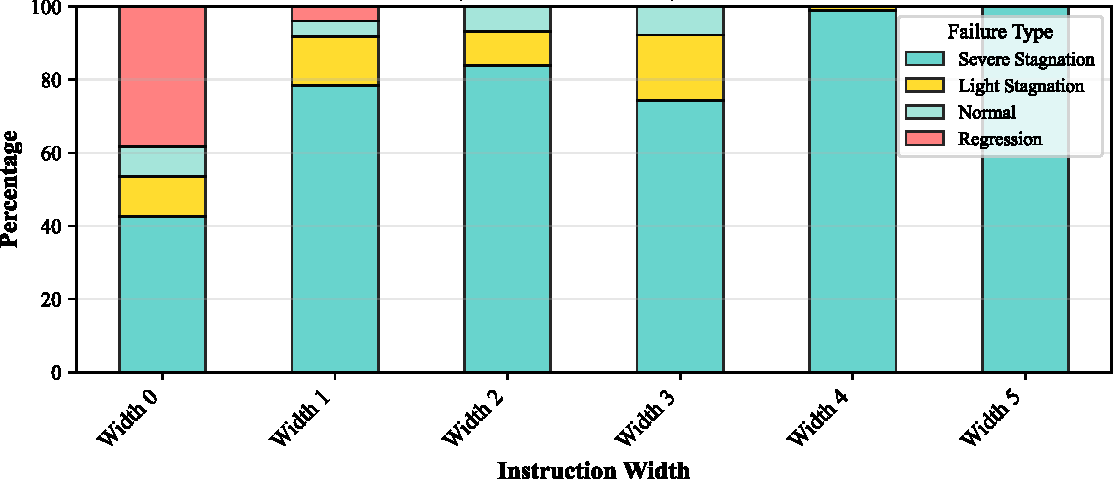
\includegraphics[width=\linewidth]{figures/q4_failure_type_dist_by_width.pdf}
    \caption{Failure type distribution across instruction widths.}
    \label{fig:failure_type_dist_by_width}
\end{figure}

\begin{figure}[H]
    \centering
    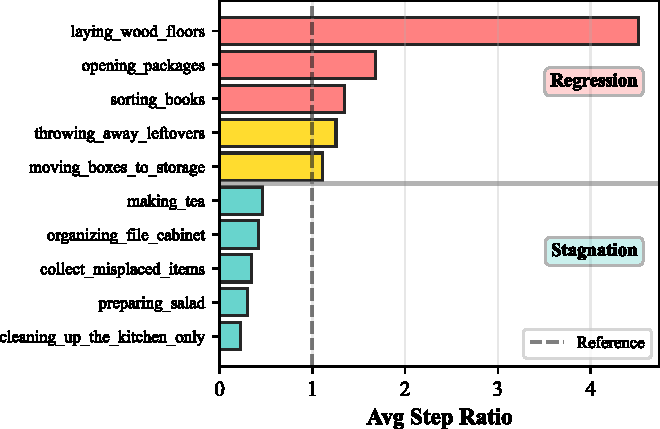
\includegraphics[width=\linewidth, keepaspectratio]{figures/q4_failure_type_extreme_task_example.pdf}
    \captionof{figure}{Low-width but long task horizon (e.g., laying woods) tends to cause regression, while high-width stagnates.}
    \label{fig:q4_failure_modes}
\end{figure}

\subsection{More Plots for Width vs. Other Linguistic Heuristics as Metric for Language Grounding Complexity}

As shown in the correlation heatmap \Cref{fig:correlation_heatmap}, $w$ is the only metric that maintains a stable negative correlation with Success Rate across all horizons. In contrast, surface metrics like Token Count and Entity Count exhibit near-zero or even positive correlations in shorter horizons (e.g., $r=0.09$ for 1-5 steps). This confirms the Complexity Paradox: while longer, more detailed instructions (higher token/entity counts) could actually provide helpful guidance that improves SR, increasing the latent planning width ($w$) invariably degrades performance.

\begin{figure}[H]
    \centering
    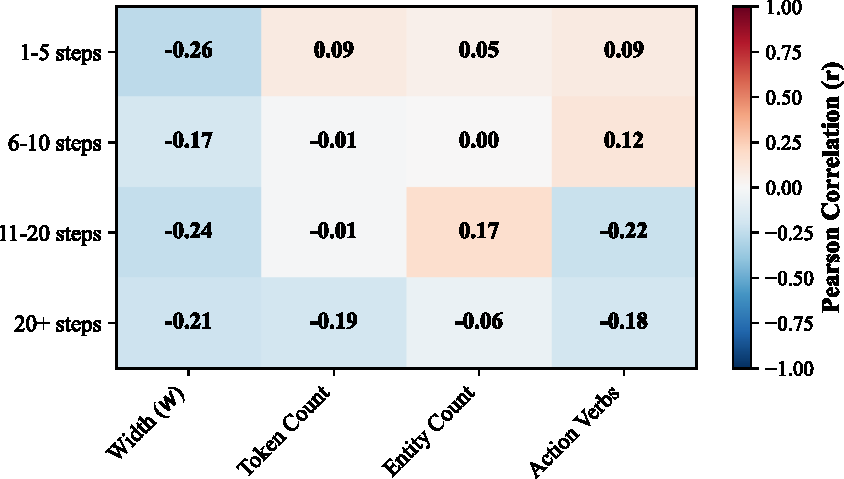
\includegraphics[width=\linewidth]{figures/q8_correlation_heatmap.pdf}
    \caption{Correlation heatmap between instruction width and other linguistic heuristics.}
    \label{fig:correlation_heatmap}
\end{figure}

Similarly, the consistency analysis in \Cref{fig:consistency_comparison} shows that $w$ possesses the lowest standard deviation ($\sigma=0.033$), indicating its predictive reliability is invariant to task horizons. Surface metrics, particularly Action Verbs ($\sigma=0.155$), are highly volatile. It also shows that $w$ provides the highest mean predictive power ($|r|=0.220$), more than doubling the predictive strength of Token Count ($0.076$) or Entity Count ($0.072$).

\begin{figure}[H]
    \centering
    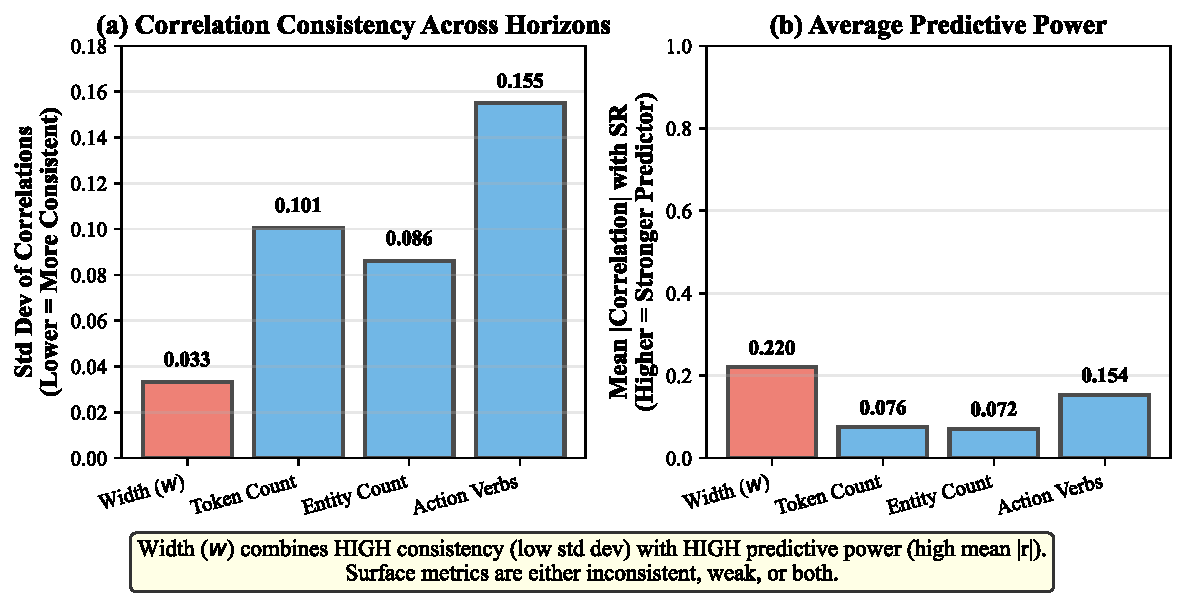
\includegraphics[width=\linewidth]{figures/q8_consistency_comparison.pdf}
    \caption{Consistency comparison between instruction width and other linguistic heuristics.}
    \label{fig:consistency_comparison}
\end{figure}

% \subsection{VLA Transformer Attention Weight Visualization}

% \begin{figure}[H]
%     \centering
%     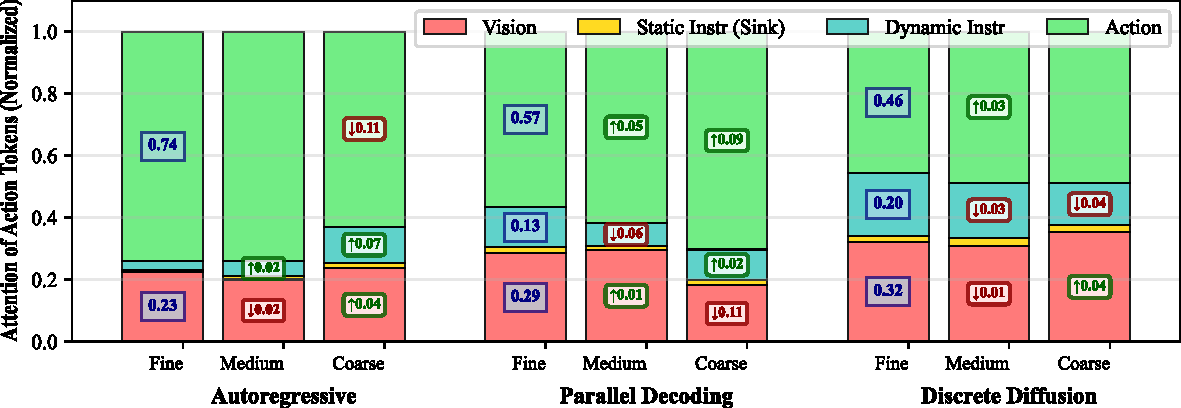
\includegraphics[width=\linewidth]{figures/q6_compare_baseline_models_attention_dist.pdf}
%     \captionof{figure}{Attention from action tokens. Self-attention dominates, followed by vision; No clear trend across granularity levels.}
%     \label{fig:attention_distribution_baseline_models}
% \end{figure}

% Attention analysis (\Cref{fig:attention_distribution_baseline_models}) reveals there is no obvious reduction in language-token attention. This suggests that in VLA architectures, maintained attention weights do not necessarily equate to language grounding, highlighting a complex dynamic that requires future investigation. 

% Nevertheless, a closer inspection of the attention distributions reveals distinct architectural behaviors and compensatory mechanisms.

% \paragraph{Autoregressive Models (Compensatory Reading).} Autoregressive generation exhibits a heavy baseline reliance on historical action tokens (accounting for $0.74$ of normalized attention in the Fine setting). Interestingly, when presented with Coarse instructions, attention to the dynamic instruction increases ($\uparrow 0.07$) while action attention decreases ($\downarrow 0.11$). This suggests a compensatory mechanism: as the rule width $w$ increases and immediate subgoals disappear, the model attempts to ground more heavily on the language prompt to search for clues.

% \paragraph{Parallel Decoding (Attending more on action modality).} This architecture demonstrates a stark multimodal decoupling under coarse instructions. The attention paid to visual tokens drops significantly ($\downarrow 0.11$) in the Coarse setting, accompanied by an increased reliance on generated action tokens ($\uparrow 0.09$). This could imply that without detailed instruction guidance at each step, parallel decoding intend to trust more on action history to decide the next actions, showing a different strategy from autoregressive models.

% \paragraph{Discrete Diffusion (Structural Stability).} Diffusion models exhibit the most balanced attention distribution, maintaining the highest baseline attention to both dynamic instructions ($0.20$) and visual features ($0.32$). Notably, this distribution remains remarkably rigid regardless of instruction granularity (with fluctuations bounded within $\pm 0.04$).


\subsection{Sample Generated Instructions by Granularity} \label{app_sec:sample_instructions}

To illustrate the qualitative differences between granularity levels, we provide five random samples for each category below. Note how Low (L) granularity explicitly specifies navigation and preconditions (e.g., move toward,'' not yet at''), while High (H) granularity focuses almost exclusively on the final state change (e.g., ``reduce the count of...''), shown in Table~\ref{tab:sample_instructions}.

\begin{table*}[ht]
\centering
\begin{minipage}{\textwidth}

\noindent\textbf{Fine Granularity (F) Samples}
\begin{tcolorbox}[colback=green!5, colframe=green!40!black]
\small
\begin{enumerate}
    \item At step 11: When the count of uncleaned plate is above 0, not yet at sink 0 and sink is off, please try to move toward sink 0.
    \item At step 8: When not yet at soap 0, not holding soap 0, the count of unwiped car is 0 and the count of rag not inside bucket is 0, please try to move toward soap 0.
    \item At step 27: When the count of chip and oatmeal sugar and vegetable oil not inside cabinet is above 0, you are at oatmeal 1 and not holding oatmeal 1, please pick up oatmeal 1.
    \item At step 15: When the count of plate not inside cabinet is above 0, you are at plate 3, the count of closed cabinet is 0 and not holding plate 3, please pick up plate 3.
    \item At step 13: When the count of fish and olive not near sink is above 0, not yet at olive 0 and not holding olive 0, please try to move toward olive 0.
\end{enumerate}
\end{tcolorbox}

\noindent\textbf{Medium Granularity (M) Samples}
\begin{tcolorbox}[colback=yellow!5, colframe=yellow!40!black]
\small
\begin{enumerate}
    \item At step 2: When the count of plate not inside cabinet is above 0, the count of closed cabinet is 0 and not holding plate 2, please pick up plate 2.
    \item At step 6: When the count of uncleaned plate is above 0, the count of dry rag is above 0 and holding rag 0, please reduce the count of dry rag.
    \item At step 9: When the count of plate not inside cabinet 0 is above 0, the count of closed cabinet is 0, the count of vegetable oil not inside cabinet 1 is 0, the count of uncleaned plate is 0 and not holding plate 0, please pick up plate 0.
    \item At step 13: When the count of book not inside box is above 0 and not holding book 2, please pick up book 2.
    \item At step 9: When the count of chip and oatmeal sugar and vegetable oil not inside cabinet is above 0, holding chip 1 and the count of closed cabinet is 0, please not holding chip 1, then reduce the count of chip and oatmeal sugar and vegetable oil not inside cabinet.
\end{enumerate}
\end{tcolorbox}

\noindent\textbf{Coarse Granularity (C) Samples}
\begin{tcolorbox}[colback=blue!5, colframe=blue!40!black]
\small
\begin{enumerate}
    \item At step 2: When the count of hamburger not inside ashcan is above 0, please reduce the count of hamburger not inside ashcan.
    \item At step 5: When the count of plate not inside cabinet is above 0 and the count of closed cabinet is 0, please reduce the count of plate not inside cabinet.
    \item At step 3: When the count of teapot not on stove is above 0, please reduce the count of teapot not on stove.
    \item At step 9: When the count of plate not inside cabinet is above 0 and the count of closed cabinet is 0, please reduce the count of plate not inside cabinet.
    \item At step 8: When the count of chip and oatmeal sugar and vegetable oil not inside cabinet is above 0 and the count of closed cabinet is 0, please reduce the count of chip and oatmeal sugar and vegetable oil not inside cabinet.
\end{enumerate}
\end{tcolorbox}

\end{minipage}
\caption{Sample generated instructions across granularity levels.}
\label{tab:sample_instructions}
\end{table*}
